\subsection{Projektumweltanalyse}

Die Projektumweltanalyse visualisiert interne und externe Beziehungen zu einem Projekt. Sie dient der Identifikation von Einflussfaktoren auf das Projekt (sowohl positive als auch negative). Anhand der Projektumweltanalyse können die Projektmitglieder die Auswirkungen der Einflussfaktoren auf das Projekt abschätzen und entsprechende Maßnahmen ergreifen. \citev{projektumweltanalyse}

\begin{figure}[H]
    \centering
    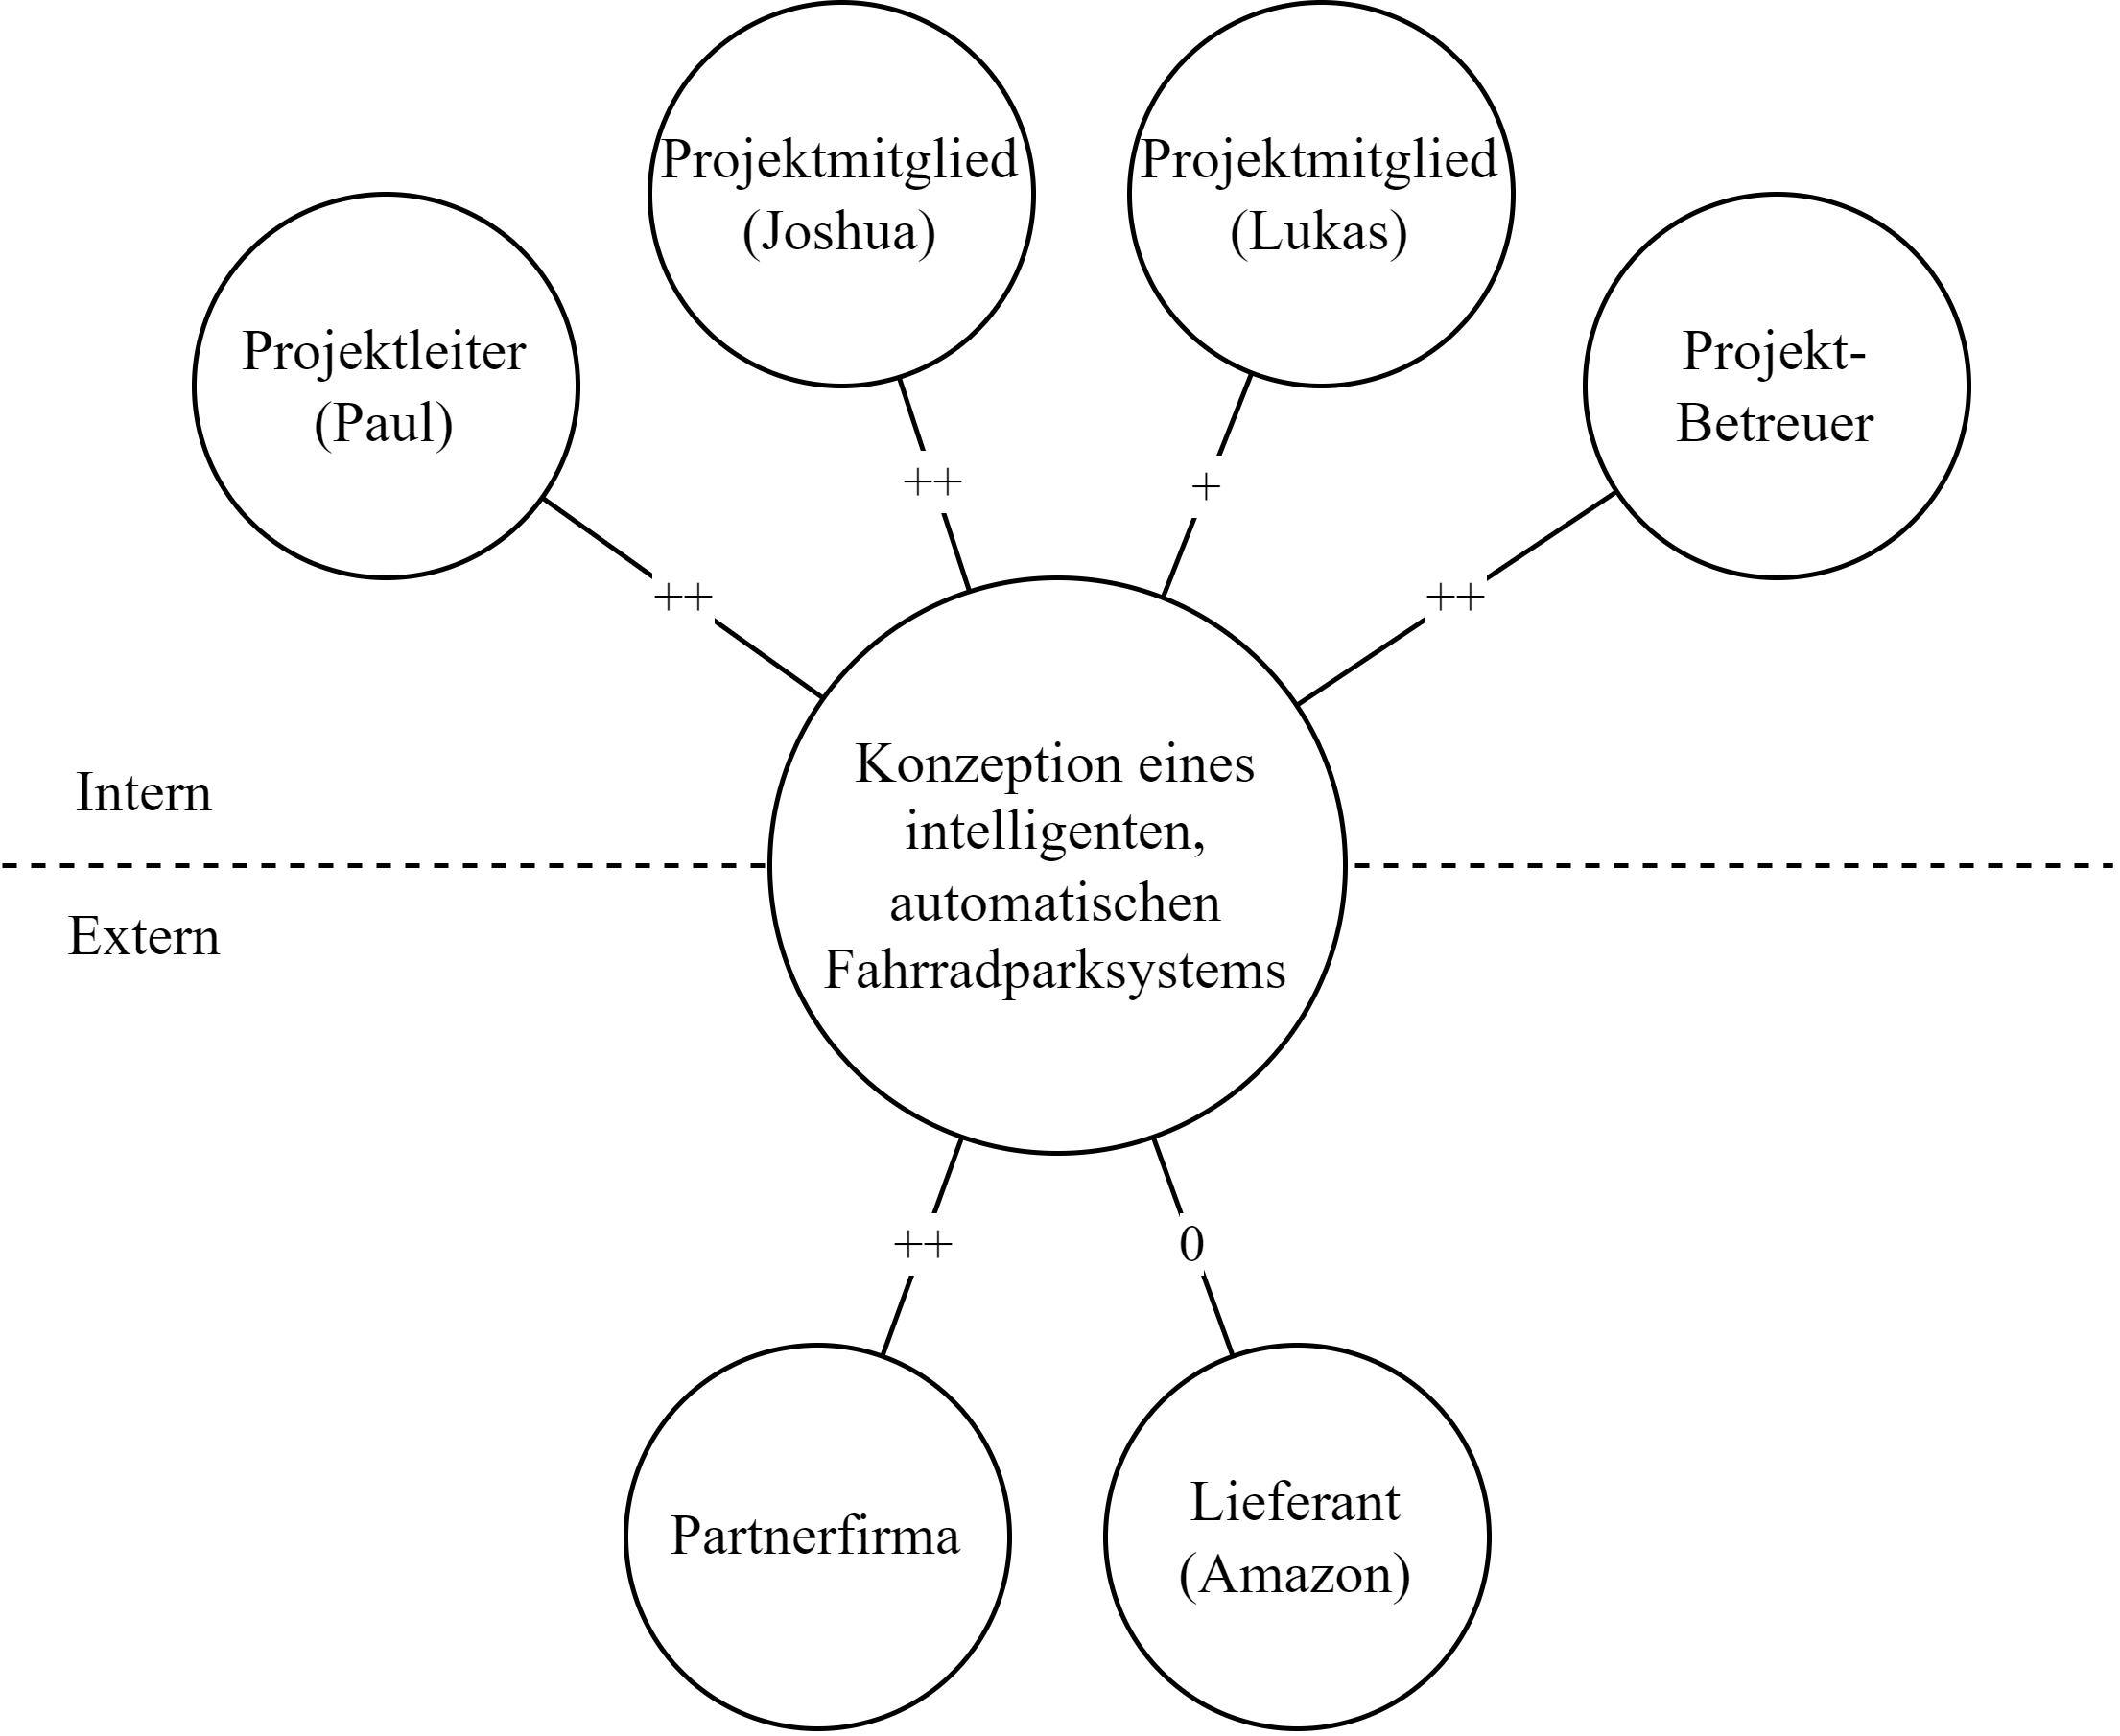
\includegraphics[width=0.8\textwidth]{images/projektumweltanalyse.png}
    \caption{Projektumweltanalyse}
    \label{fig:projektumweltanalyse}
\end{figure}

\begin{table}
    \centering
    \begin{tabular}{lp{0.3\textwidth}p{0.4\textwidth}}
        \multicolumn{3}{c}{\textbf{Projektumweltanalyse (Tabellarische Form)}}                                                 \\
        \toprule
        \textbf{Umwelt}             & \textbf{Risiko}                         & \textbf{Maßnahme Strategie}                    \\
        \midrule
        Projektmitglied (Lukas) [0] & Erledigt Aufgaben nicht / Unverlässlich & \begin{itemize}
                                                                                    \item Lukas übernimmt keine kritischen Aufgaben
                                                                                    \item Geringeres Arbeitspensum
                                                                                    \item Pufferzeiten einplanen
                                                                                \end{itemize} \\
        Lieferant (Amazon) [0]      & Lieferzeit zu lang oder verpätet        & \begin{itemize}
                                                                                    \item Pufferzeiten einplanen
                                                                                    \item Frühzeitig bestellen
                                                                                \end{itemize}                    \\
        \bottomrule
    \end{tabular}
    \caption{Projektumweltanalyse (Tabellarische Form)}
    \label{tab:projektumweltanalyse}
\end{table}